% -*- root: ../../main.tex -*-
\section{Esempi D'Uso}
Una volta avviati tutti i componenti del cluster (Client e Servers): sarà necessario attendere che la schermata si aggiorni con le informazioni iniziali dei vari server.

La schermata principale con i suoi relativi comandi è la seguente:

\begin{figure}[H]
	\centering
	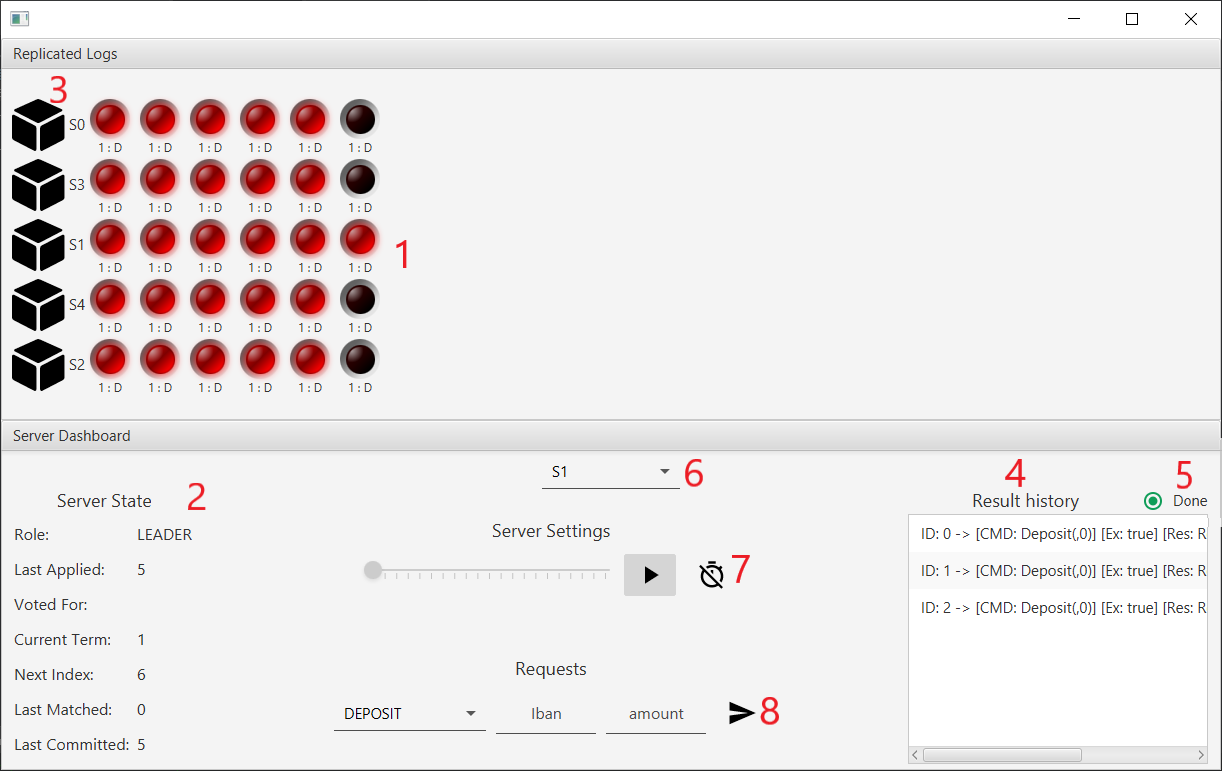
\includegraphics[width=0.99\columnwidth]{usageExample/mainView}
	\caption[usageExampleCaption]{Screenshot della schermata principale durante il normale funzionamento. In rosso vediamo elencati tutti gli elementi fondamentali della Gui.}
	\label{fig:figure15}
\end{figure}

Procediamo nel descrivere tutti i principali elementi presenti nella schermata:
\begin{enumerate}
	\item \texttt{Log di tutti i server}: 
  Ogni server ha un \textbf{log} rappresentato da un insieme di \textbf{entry}, ogni entry è costituita da un term(un numero) e un comando(\texttt{Deposit}, \texttt{Withdraw} e \texttt{Get Balance}) rappresentato dalle lettere: \texttt{D}, \texttt{W} e \texttt{G}. Inoltre ogni entry del log ha un colore, nero o rosso. Dove rosso significa che l'entry ha ancora ricevuto il commit, nero che non lo ha ricevuto.
	\item \texttt{Stato del server selezionato:}
  In questo riquadro sono riportate le informazioni più importanti del server attualmente selezionato.
	\item \texttt{Colonna dei server:}
  Nella colonna sottostante per ogni server è riportato il nome, e lo stato del log allineato in riga.
	\item \texttt{Storico risultati/richieste:}
  In questa textarea sono riportate tutte le richieste e i relativi risultati (se presenti), inoltre nella stessa area sono riportati anche le richieste pendenti.
	\item \texttt{Tasto per cambio storico:}
  Tramite questo tasto è possibile passare dalla visualizzazione dello storico risultati, alla visualizzazione delle richieste pendenti.
	\item \texttt{Selezione server:}
  Tramite la combobox è possibile selezionare un server del cluster.
	\item \texttt{Comandi server selezionato:}
		I tre comandi disponibili sono tutti indipendenti tra loro, da sinistra verso detra i significati sono:
		\begin{itemize}
			\item \texttt{Slider:} 
      Lo slider parte da zero e identifica la percentuale che il server selezionato ha di perdere ogni messaggio ricevuto.
			Il valore viene impostato una volta che lo slider viene rilasciato, e non durante lo spostamento; inoltre i valori vengono approssimati di cinque in cinque.
			\item \texttt{Start/Stop:}
      Il tasto start/stop permette di bloccare e riprendere l'esecuzione del server selezionato. 
			\item \texttt{Timeout:}
      Tramite il tasto di timeout è possibile inviare un messaggio al server selezionato.Questo messaggio farà scattare il \textbf{Timer} del server; che quindi si comporterà diversamente in base al suo stato attuale(Follower, Leader o Candidate). 
		\end{itemize}
		Ogni comando viene inviato al server selezionato in via prioritaria, e quindi viene recapitato il prima possibile; indipendentemente dallo stato del server selezionato. 
	\item \texttt{Interfaccia di invio richieste}:
		In questo punto è possibile inviare nuove richieste da parte del \texttt{Client} verso il \texttt{Server} attualmente selezionato.
		Una volta scelto il comando tra: Deposit, withdraw e get balance; sarà necessario inserire il codice \texttt{iban} dell'conto e l'importo per la specifica operazione.
		Infine è possibile inviare la richiesta, in caso non si selezioni nulla vengono scelti iban nullo e valore zero.	
\end{enumerate}
Non è possibile procedere con il lancio di alcun comando fino a quando sono presenti le scritte \textbf{undefined} nello stato del server.

In figura: \ref{fig:figure15} è riportato un esempio in cui il server S1, ovvero l'attuale, ha diffuso cinque entry e stava procedendo alla diffusione dei messaggi di commit con il prossimo \texttt{Earthbeat}. Ma è stato bloccato dal \texttt{Client}.
Possiamo notare come tutte le entry hanno lo stesso term, quindi sono state diffuse durante il regno del primo leader.
Le entry da lui diffuse non sono ancora committate, e dato il suo mancare possiamo certamente aspettarci l'insorgere di un nuovo \textbf{Leader}, che si metterà in attesa di nuove entry da diffondere.
